\section{Versuchsaufbau}
\label{sec:Aufbau}

Der verwendete Versuchsaufbau ist in \autoref{fig:aufbau} abgebildet.

\begin{figure}[H]
    \centering
    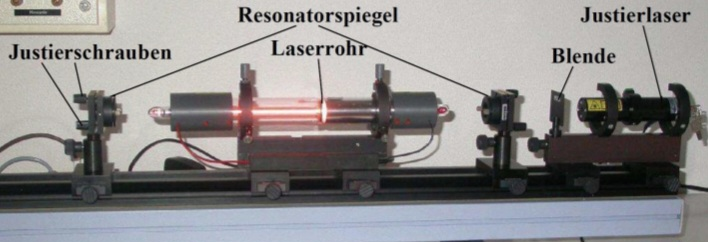
\includegraphics[width=\textwidth]{data/Aufbau.jpg}
    \caption{Aufbau des Versuches \cite{Anleitung61}.}
    \label{fig:aufbau}
\end{figure}

\noindent
Sämtliche für die Justierung und folgenden Messungen verwendeten Bauteile befinden sich auf einer optischen Schiene. Es wird als Justierlaser ein grüner Laser mit einer
Wellenlänge von $\lambda = 532\, \si{\nano\metre}$ und einer Leistung von $P = 0,2\, \si{\milli\watt}$ verwendet. Zu beiden Seiten des He-Ne Laserrohrs befindet sich jeweils
ein Resonatorspiegel. Das Laserrohr hat hierbei eine Länge von $l = 408\, \si{\milli\metre}$ und einen Durchmesser von $d = 1,1\, \si{\milli\metre}$.
\noindent
Für die verschiedenen Messungen stehen außerdem eine Photodiode, ein Polarisationsfilter und Gitter verschiedener Konstanten zur Verfügung, die nach Bedarf ebenfalls auf der
optischen Schiene befestigt werden können. 


\section{Durchführung}
\label{sec:Durchführung}

Bevor mit den verschiedenen Messungen begonnen werden kann muss zunächst der Laser justiert werden. Hierfür wird der Justierlaser verwendet um die Feineinstellungen an
den Spiegeln vorzunehmen. Die Leistung des Lasers wird dabei von einer Photodiode gemessen. Die Justierung ist abgeschlossen, sobald man für die Lesitung des Lasers ein
Maximum erreicht.


\subsection{Messung der Stabilität}

Für die Bestimmung der Stabilität wird erneut die Leistung des Lasers mit Hilfe der Photodiode gemessen. Diese Messung wird allerdings mehrmals für größer werdende
Spiegelabstäde wiederholt. Dabei werden für jeden Abstand die Spiegel nachjustiert, um die jeweils größte Laserleistung zu erreichen. Dies wird wiederholt, bis
ein Abstand erreicht wurde, bei dem keine Intensität messbar ist. Es werden dabei sowohl ein Konkav-Konkav-Resonator als auch ein Plan-Konkav-Resonator verwendet.


\subsection{Messung des Frequenzspektrums}

Da für die Bestimmung der Schwebungsfrequenzen ebenfalls verschiedene Resonatorlängen notwendig sind, ist es sinnvoll, diese Messung parallel zur Bestimmung der Stabilität
durchzuführen. Hierfür muss lediglich bei jeder Resonatorlänge die Photodiode durch eine schnelle Photodiode ausgewechselt werden. Diese ist an einen Spektrumsanalysator
angeschlossen, an dem dann die Frequenzpeaks abgelesen werden können. 


\subsection{Messung des TEM-Moden}

Zur Vermessung der TEM-Moden wird ein als Modenblende fungierender Wolframdraht zwischen Laserrohr und Spiegel gespannt. Dieser wird dann so ausgerichtet, dass
die verschiedenen Moden auf dem Schirm sichtbar werden. Um die Moden vermessen zu können, muss der Strahlendurchmesser mittels einer Streulinse vergrößert werden.
Mit Hilfe einer Lochblende und Photodiode kann dann die Intensitätsverteilung der Moden sekrecht zur optischen Achse vermessen werden.


\subsection{Messung der Polarisation}

Um die Polarisation zu bestimmen wird zwischen Resonatorspiegel und Photodiode ein Polarisationsfilter eingebaut. Dabei wird für volle 360° in jeweils 10°-Schritten
die Intensität mit der Photodiode gemessen. 


\subsection{Messung der Wellenlänge}

Für die Bestimmung der Wellenlänge werden verschiedene Gitter mit Gitterkonstanten von $g = 80\, \frac{\text{Linien}}{\si{\milli\metre}}$,
$g = 100\, \frac{\text{Linien}}{\si{\milli\metre}}$,
$g = 600\, \frac{\text{Linien}}{\si{\milli\metre}}$ und $g = 1200\, \frac{\text{Linien}}{\si{\milli\metre}}$ verwendet. Es werden für die vier Beugungsmuster
jeweils die Abstände der Maxima zum Hauptmaximum, zusammen mit dem Abstand des Gitters zum Schirm gemessen, um daraus die Wellenlänge zu berechnen.
